\chapter{Универсальная аппроксимация в 1D}
\label{sec:universal_approximation}

\begin{supportbox}{Об этой главе}
Хотя формальное доказательство теоремы об универсальной аппроксимации выходит за рамки этой книги, полезно получить интуитивное представление о том, как такие доказательства могут быть построены. В этом приложении мы следуем и расширяем визуальные интуиции из главы онлайн-книги М. Нильсена 2019 года,\footnote{\url{http://neuralnetworksanddeeplearning.com/chap4.html}} к которой мы отсылаем для расширенного обсуждения (и некоторых интерактивных визуализаций), особенно для случая многомерных входов.
\end{supportbox}

Мы сосредоточимся на оригинальной теореме аппроксимации Цыбенко \cite{cybenko1989approximation}, которая рассматривает модели с одним скрытым слоем с сигмоидальными функциями активации. Мы также ограничиваем анализ функциями с одним входом и одним выходом, которые можно легко визуализировать. Рассуждения можно распространить на другие функции активации и на более высокие размерности.

План этого визуального доказательства относительно прост: 

\begin{enumerate}
\item В качестве первого шага мы покажем, как вручную установить веса модели с одним нейроном в скрытом слое для аппроксимации ступенчатой функции.
\item Затем мы покажем, как добавление еще одного блока в скрытый слой позволяет аппроксимировать любую функцию, которая является постоянной на небольшом интервале и нулевой везде вне его (мы называем эти интервальные функции «бин»-функциями). 
\item Наконец, мы опишем простую процедуру для аппроксимации общей функции, сначала разбив ее на бины до желаемой точности, а затем добавляя столько нейронов, сколько необходимо для аппроксимации всех бинов по очереди. Для $m$ бинов мы получаем сеть с $2m$ нейронами. Для общей функции с несколькими входами это число будет расти экспоненциально с числом измерений, что делает доказательство неконструктивным в практическом случае.
\end{enumerate}

\section{Аппроксимация ступенчатой функции}

Для начала рассмотрим один нейрон в скрытом слое, и в этом случае мы можем записать уравнение сети как (игнорируя член смещения на выходе, поскольку он не помогает в нашем выводе):
%
$$
f(x)=a\sigma(wx+s)
$$
%
Для целей визуализации мы перепишем это, добавив знак минус к смещению, и вынесем множитель за скобки для всего входа $\sigma$ (два варианта, очевидно, эквивалентны):
%
\begin{equation}
f(x) = \eqnmarkbox[drawred]{node}{a}\sigma(\eqnmarkbox[drawgreen]{node2}{w}(x-\eqnmarkbox[drawblue]{node3}{s}))
\label{eq:proof_1}
\end{equation}
\annotate[yshift=-1em]{below,left}{node}{Амплитуда}
\annotate[yshift=-1em]{below,right}{node2}{Наклон}
\annotate[yshift=-1em]{below,right}{node3}{Сдвиг}

\vspace{1em}
Это похоже на «настраиваемый» вариант сигмоиды, который мы вводим в Разделе \ref{sec:activation_functions}. В частности, в этой формулировке $\color{drawred}a$ контролирует амплитуду сигмоиды, $\color{drawgreen}w$ контролирует наклон, а $\color{drawblue}s$ сдвигает функцию на фиксированную величину.

\begin{SCfigure}
    \centering
    \hspace{1em}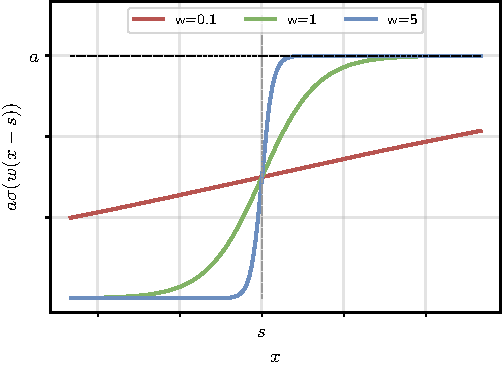
\includegraphics[width=0.5\textwidth]{images/tunable_sigmoid.pdf}
    \caption{Сеть с одним нейроном в скрытом слое можно представить как сигмоиду с управляемым наклоном, центром и амплитудой. Здесь мы показываем пример, где мы фиксируем амплитуду и центр, но изменяем наклон.}
    \label{fig:tunable_sigmoid}
\end{SCfigure}
%
Мы показываем на Рисунке \ref{fig:tunable_sigmoid} несколько графиков \eqref{eq:proof_1}, где мы фиксируем $a$ и $s$, изменяя $w$. Как видно, при увеличении $w$ наклон становится круче. Зафиксировав его на очень большой константе (скажем, $w=10^4$), мы получаем очень хорошую аппроксимацию ступенчатой функции, для которой мы можем контролировать положение ступеньки (параметр $s$) и амплитуду (параметр $a$), как показано на Рисунке \ref{fig:step_function}.

\begin{figure}
    \centering
    \begin{subfigure}[b]{0.32\textwidth}
    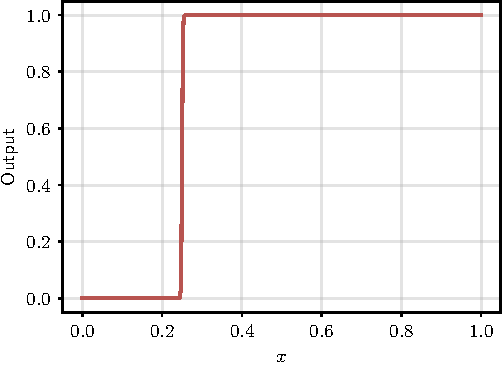
\includegraphics[width=0.95\textwidth]{images/step_function.pdf}
    \caption{1 нейрон}
    \label{fig:step_function}
    \end{subfigure}
    \hfill
    \begin{subfigure}[b]{0.32\textwidth}
    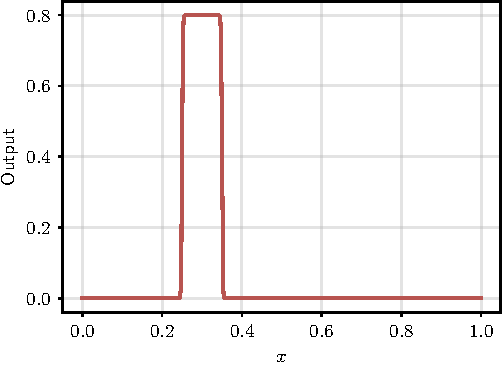
\includegraphics[width=0.95\textwidth]{images/bin.pdf}
    \caption{2 нейрона}
    \label{fig:bin_function}
    \end{subfigure}
    \begin{subfigure}[b]{0.32\textwidth}
    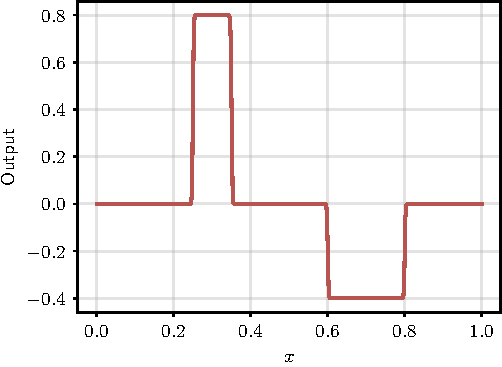
\includegraphics[width=0.95\textwidth]{images/bin_2.pdf}
    \caption{4 нейрона}
    \label{fig:bin_function_2}
    \end{subfigure}
    \caption{(a) Нейронная сеть с одним входом, одним скрытым нейроном и одним выходом может аппроксимировать любую ступенчатую функцию (здесь показано с $a=1$ и $s=0.3$). (b) С двумя скрытыми нейронами и одним выходом мы можем аппроксимировать любую функцию, которая является постоянной на небольшом интервале. (c) С четырьмя нейронами мы можем аппроксимировать любую функцию, которая является кусочно-постоянной на двух ненулевых интервалах. Обратите внимание, что бины могут быть отрицательными, если определить отрицательную амплитуду.}
\end{figure}

\section{Аппроксимация постоянной функции}

Если мы добавим второй нейрон с противоположной амплитудой (и немного сдвинутым положением), мы можем аппроксимировать функцию, которая является постоянной на небольшом интервале (мы называем ее «бин»-функцией). Определив ширину $\Delta$, мы можем записать:

\begin{equation}
f(x) = a\sigma\left(w\left(x-\eqnmarkbox[drawred]{node}{s -\frac{\Delta}{2}}\right)\right)  -a\sigma\left(w\left(x-\eqnmarkbox[drawgreen]{node2}{s+\frac{\Delta}{2}}\right)\right)
\label{eq:proof_2}
\end{equation}
\annotate[yshift=-1em]{below,left}{node}{Подняться [опуститься] в $s-\frac{\Delta}{2}$}
\annotate[yshift=-1em]{below,right}{node2}{Опуститься [подняться] в $s+\frac{\Delta}{2}$}

\vspace{1em}
где мы напоминаем, что $w$ теперь является большой константой, например, $10^4$. \eqref{eq:proof_2} описывает функцию (эквивалентную модели с одним скрытым слоем с двумя нейронами), которая увеличивается на $a$ в $s-\frac{\Delta}{2}$, является постоянной со значением $f(x)=a$ над интервалом $\left[s-\frac{\Delta}{2}, s+\frac{\Delta}{2}\right]$, а затем уменьшается до $0$. Пример показан на Рисунке \ref{fig:bin_function}.

Для дальнейшего мы можем переписать предыдущую функцию как $f(x; a, s, \Delta)$, чтобы подчеркнуть зависимость от трех параметров $a$, $s$ и $\Delta$.

\section{Аппроксимация кусочно-постоянной функции}

Поскольку $f_{a, s, \Delta}(x)$ фактически равна $0$ вне соответствующего интервала, две функции, определенные на непересекающихся интервалах, не будут влиять друг на друга, т.е. «бин»-функция, которую мы только что определили, сильно локализована. Следовательно, добавив два дополнительных нейрона в скрытый слой, мы можем определить функцию, которая является постоянной на двух отдельных интервалах (пример которой показан на Рисунке \ref{fig:bin_function_2}):
%
$$
f(x)=f(x;a_1,s_2,\Delta_1)+f(x;a_2,s_2,\Delta_2)
$$
%
Остальная часть доказательства теперь тривиальна и заключается в разбиении функции, которую мы хотим аппроксимировать, на множество небольших интервалов. Для любой (непрерывной) функции $g(x)$ на интервале (который мы для простоты предполагаем $[0,1]$), мы сначала разбиваем входную область на $m$ равноотстоящих интервалов, где $m$ контролирует точность аппроксимации (чем больше $m$, тем лучше аппроксимация). Следовательно, $i$-й бин охватывает интервал:
%
$$
B_i = \left[\frac{i}{m}-\frac{\Delta}{2}, \frac{i}{m}+\frac{\Delta}{2}\right]
$$
%
где $\Delta$ — это размер каждого бина. Для каждого бина мы вычисляем среднее значение $g(x)$ внутри самого интервала:
%
$$
g_i = \frac{1}{\Delta}\int_{x \in B_i} g(x)dx
$$
%
Наконец, мы определяем сеть с $2m$ нейронами в скрытом слое, по два на каждый бин. Каждая бин-функция центрирована в бине и принимает значение $g_i$:
%
\begin{equation}
f(x)=\sum_{i=1}^m f\left(x; \eqnmarkbox[drawgreen]{node2}{g_i}, \eqnmarkbox[drawred]{node}{\frac{i}{m}},\Delta\right)
\label{eq:proof_3}
\end{equation}
\annotate[yshift=-1em]{below,right}{node}{$i$-й бин центрирован в $\frac{i}{m}$}
\annotate[yshift=-1em]{below,left}{node2}{(Приближенное) постоянное значение}

\newpage
Мы показываем на Рисунке \ref{fig:sin_approximation} пример такой аппроксимации в случае $g(x)=\frac{\sin(x)}{x}$ для возрастающего числа бинов ($m=5$, $m=15$, $m=50$). Должно быть ясно, что СКО обратно пропорциональна $m$, и мы можем уменьшать ошибку сколько угодно, просто увеличивая разрешение аппроксимации.

\begin{figure}[t]
    \centering
    \begin{subfigure}[b]{0.32\textwidth}
    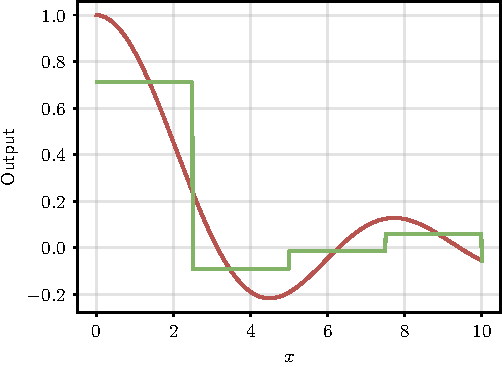
\includegraphics[width=0.95\textwidth]{images/sin_approximation_5.pdf}
    \caption{5 бинов}
    \end{subfigure}
    \hfill
    \begin{subfigure}[b]{0.32\textwidth}
    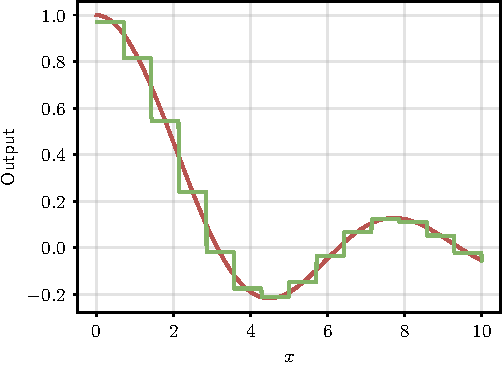
\includegraphics[width=0.95\textwidth]{images/sin_approximation_15.pdf}
    \caption{15 бинов}
    \end{subfigure}
    \hfill
    \begin{subfigure}[b]{0.32\textwidth}
    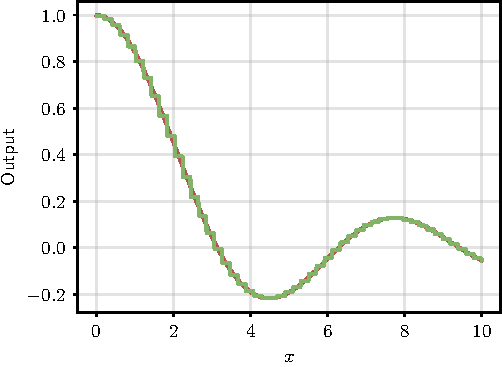
\includegraphics[width=0.95\textwidth]{images/sin_approximation_50.pdf}
    \caption{50 бинов}
    \end{subfigure}
    \hfill
    \caption{Аппроксимация $g(x) = \frac{\sin(x)}{x}$ в $[0,10]$ с (a) $m=5$, (b) $m=15$ и (c) $m=50$ бинами. Исходная функция — красная, аппроксимация \eqref{eq:proof_3} — зеленая. Среднеквадратичная ошибка в трех случаях экспоненциально уменьшается (приблизительно $0.02$, $0.002$ и $0.00016$).}
    \label{fig:sin_approximation}
\end{figure}

Аналогичные рассуждения можно применить к многомерным входам и различным функциям активации.\footnote{\url{http://neuralnetworksanddeeplearning.com/chap4.html}}